\chapter{Agentul DQN}

\section{Contextul curent}
În ciuda popularității sale accentuate și al bazei mari de jucători, preponderent observată în ultimii ani, jocul Monopoly nu s-a bucurat de o prezență impunătoare în cazul studiilor efectuate pentru învățarea automată. Multe studii timpurii \cite{mdp_monopoly_1}, \cite{mdp_monopoly_2} și-au bazat cercetarea ca pură definire a abordării modelării jocului ca un proces Markov, iar o lucrare mai recentă \cite{mdp_monopoly_3} a concretizat efortul anterior și ca un proces decizional Markov.

O încercare de abordare hibridă a putut fi observată în cadrul lucrării \cite{hybrid_monopoly}, unde autorii s-au remarcat prin folosirea metodelor algoritmice în cadrul acțiunilor nefavorabile învățării prin întărire, precum cele care ar fi necesitat o colectare îndelungată de date, dat fiind caracterul lor sporadic, precum decizia utilizării unui cartonaș de ieșit din închisoare. Totuși, abordarea lor presupunea folosirea unei singure rețele pentru antrenarea și prezicerea acțiunilor, lucru ce poate îngreuna acuratețea și perspicacitatea deciziilor.

Cercetarea condusă a demonstrat că nicio lucrare menționată anterior sau precursoare al acestora nu a considerat o arhitectură bazată pe mai multe rețele neuronale atribuite fiecărei acțiuni. Totodată se remarcă lipsa unei abordări a unui sistem expert, menite să reducă timpul de antrenare și îmbunătățească abilitatea agentului de învățare \cite{expert_learning}. Conform programului de antrenare în vederea găsirii unei abordări dinamice pentru jocul GO \cite{alphago}, învățarea supervizată folosind o bază de date de 30 de milioane de experiențe colectate, au reușit să reducă semnificativ timpul de antrenare inițială al modelului.

\section{Arhitectura hibridă}
\subsection{Motivația pentru arhitectura hibridă}
Așa cum am văzut până acum, proiectarea unei politici optime este imprecisă și nefezabilă, din punct de vedere al timpului investit în gândirea și proiectarea algoritmului dar și a testării și evaluării sale obiective. De aceea lucrarea curentă își propune evidențierea și utilitatea unei abordări hibride în scopul obținerii unor rezultate excelente care să depășească cu un proces remarcant agenții algoritmici.

Introducerea unei astfel de decizii de design își are fundamentele pe avantajele conferite:
\begin{itemize}
    \item \textbf{Specializarea pe domenii specifice}: Ne putem focaliza pe implementarea rețelelor neuronale pentru acele metode fezabile și putem folosi implementarea algoritmică pentru celelalte metode.
    \item \textbf{Eficiența antrenamentului}: Vom putea reduce timpul necesar și complexitatea codului, având în vedere antrenamentul metodelor fezabile.
    \item \textbf{Flexibilitate arhitecturală}: Posibilitatea de a folosi sau nu a metodelor pe baza de rețele neuronale independente.
\end{itemize}

\subsection{Integrarea cu agentul strategic}
Agentul DQN este implementat ca o extensie a agentului strategic, folosind tehnica de moștenire din Python \cite{python_inheritance}, pe baza căreia, toate metodele sunt public accesibile și folosibile, având posibilitatea de a decide modul de operare curent al fiecărei acțiuni, așadar putând decide modul de tranziționare graduală de la algoritmii clasici la învățarea automată.

Abordarea moștenirii oferă posibilitatea de asigurare a tratării excepțiilor prin întreprinderea metodelor părinte, fapt ce asigură un comportament complet funcțional. De asemenea integrarea și adăugarea ulterioară a metodelor se poate face treptat, fără a avea nevoie de o structură monolitică a compunerii agentului, folosind metodele deja expuse, ulterior înlocuindu-le o versiune îmbunătățită. Testarea metodelor devine și ea trivială, fiind facilitatea de izolare a metodei folosite și observarea procentului de implicare în rata de câștig.

\subsection{Separarea deciziilor}
Deși o componentă importantă, ce reușește să rezolve și îmbunătățească numeroase conflicte de interes, schimbul rămâne o acțiune incertă și doar un refugiu în privința incrementării averii din joc. Datorită complexității ridicate de encodare a unei oferte de schimb, a proiectării unei funcții optime de recompensă și a frecvenței reduse de observații, metodele aferente schimbului au fost complet excluse din faza învățării automate și tratate prin folosirea metodelor părinte.

De asemenea, tratarea metodei de recuperare din faliment a fost preluată din părinte, aceasta având o rată mică de apariție în joc, dar și datorită numeroaselor aspecte implicate, precum decizia de ierarhizare a pașilor în rezolvarea falimentului, prioritizare obiectivelor de scurtă durată și influența rezolvării conflictelor financiare.

Celelalte metode prezentate în tabelul \ref{fig:player_interface_methods} vor fi implementate folosind paradigme învățării automate, prin rețele neuronale de tipul Q (Deep Q-Networks, DQN). În urma testelor efectuate, s-a realizat că pentru anumite metode de modificare a posesiunilor, rețelele nu reușeau să surprindă eficient pericolele viitoare ale deciziilor curente, precum ipotecarea sau vânzarea caselor/hotelurilor. Așadar s-a considerat utilizarea unei abordări mixte, prin executarea acțiunii rețelei, doar când metoda părinte ar fi considerat benefică efectuarea acțiunii. Astfel, s-a observat o creștere de 33\% comparativ cu o abordare statică ce considera doar rezultatul rețelei.

Considerentele ce ar putea fi implicate sunt greu de concretizat, dar presupunerea proprie observată în urma experimentelor arată că rețeaua nu a reușit să capteze în totalitate consecințele viitoare ale unei acțiuni distructive.

\section{Rețele de tipul Q}
Într-un mediu cu număr de stări și acțiuni predefinit, relativ mic, se pot folosi matrici bidimensionale pentru maparea valorilor Q pentru fiecare pereche de stare și acțiuni, astfel construindu-se o reprezentare detaliată a politicii optime. Din păcate, într-un mediu dificil de reprezentat și configurat, cu un număr impunător de tranziții de stări și acțiuni, această mapare ar fi imposibil de realizat datorită dimensiunilor reduse ale memoriei, dar și din cauza timpului îndelungat necesar explorării tuturor tranzițiilor pentru generarea unei politici optime. Ca și referință putem avea în vedere un joc de șah, în care s-a estimat că totalitatea stărilor posibile ar fi aproximativ $10^{43}$ \cite{shannon1950chess}, un număr extraordinar, comparativ cu puterea de calcul și stocare actuală.

Astfel, rețelele neuronale sunt folosite pentru replicarea mapării, generând o funcție de mapare, în loc să păstreze valorile mapate. Acest lucru simplifică spațiul de stocare necesar, fiind o alternativă viabilă în cadrul spațiilor vaste de acțiune. Acestea au ca argument (input) reprezentarea vectorială a stării curente (embedding) și oferă aproximarea valorii Q ca și rezultat (output).

\subsection{Encodarea stării. Spațiul de acțiuni}\label{state-embeding}
În vederea realizării encodării stării, s-a plecat de la datele avute la dispoziție și expuse de reprezentarea oferită de GameState. Astfel s-a decis încorporarea lor într-o formă vectorială, într-un spațiu real cu 100 de dimensiuni. Reprezentarea dimensională a fost făcută doar pentru regulile predefinite, plecând cu presupunerea că vor exista doar doi jucători pe parcursul oricărui joc. Aceasta s-a făcut într-o formă alternativă, plecând cu informația agentului curent, urmată de informația oponentului, secvențial pentru fiecare categorie, după cum urmează:
\begin{itemize}
    \item \textbf{Informațiile jucătorilor (8 caracteristici)}: pozițiile pe tablă, balanțul cash, statutul libertății, cărțile de ieșire din închisoare.
    \item \textbf{Indicatori al monopolurilor (48 de caracteristici)}: deținerea proprietăților, al caselor/hotelurilor, al proprietăților ipotecate.
    \item \textbf{Contextualizare strategică (44 de caracteristici)}: gradul de progres al jocului, gradul de apreciere al utilităților, numărul turelor în închisoare, etc.
\end{itemize}

\begin{figure}[H]
    \centering
    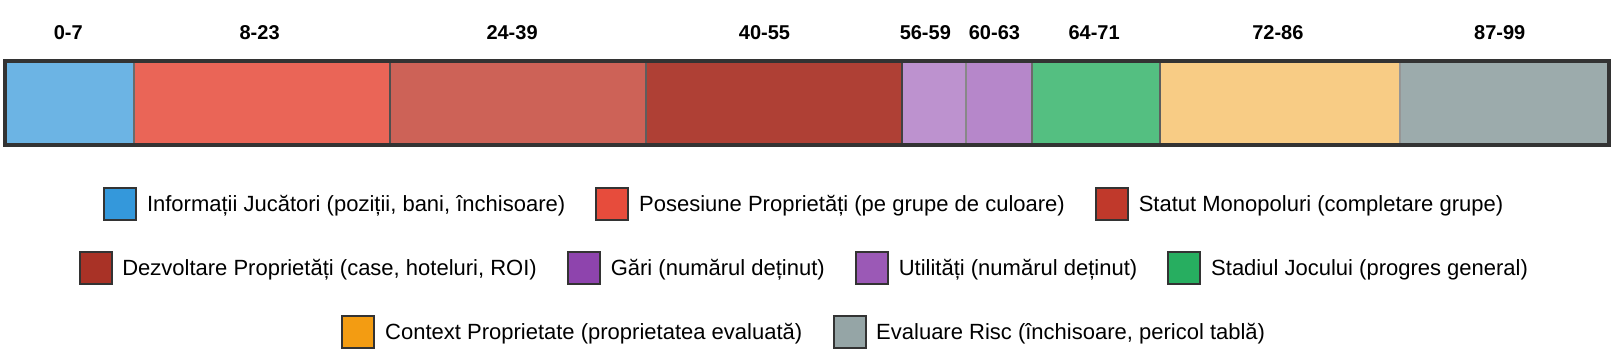
\includegraphics[width=16cm]{images/vector_visualizer.png}
    \caption{Vizualizarea distribuției informației în encodarea stării}
    \label{fig:state-distribution}
\end{figure}

Conform observațiilor recente \cite{drl_normalization_benefits}, normalizarea datelor în procesul de preprocesare aduce multiple beneficii precum reducerea pierderilor datorate unei înclinații (bias) nefavorabile în mediu, cât și asigurarea unei convergențe mai bune în scopul obținerii unei politici optime.

Rezultatele observate folosind normalizarea datelor în procesul de embedding, au fost comparate cu o abordare nenormalizată, observându-se atât un rezultat superior în cazul ratei de câștig, cât și o politică mai bună în cazul testelor cu un agent uman.

Limitele folosite în marginire au fost fie evidente, precum numărul maxim de cărți de ieșit din închisoare (2), număr predefinit de regulile jocului, fie alese în urma rulării mai multor mii de jocuri și colectării de date, având o marjă de incrementare considerabilă (aproximativ 30\%) cu scopul evitării și minimizării utilizării de valori supraunitare. De exemplu balanța cash a fiecărui jucător a fost raționalizată în funcție de o sumă maximă de 5.000₩.

Asemănător acțiunilor prezentate în tabelul \ref{fig:player_interface_methods}, dimensionalitatea metodelor a fost păstrată integral, excepție făcând metodele de ipotecare și dezipotecare, care au avut în cazul implementării dimensiunea de 40, corespunzătoare fiecărei căsuțe de pe tablă. Aceasta s-a realizat în urma observării unui rezultat net inferior păstrării numărului de 22 de celule aferent tuturor proprietăților cumpărabile. Ipoteza emisă este greu de justificat, dar este probabil ca rețeaua să prefere o discretizare apropiată de factorul de normalizare folosit anterior pentru raționalizarea căsuțelor și a pozițiilor.

\section{Designul rețelelor neuronale}
\subsection{Rețele multiple}
O contribuție majoră a acestei implementări a fost folosirea multiplelor rețele neuronale pentru fiecare tip de decizie. În lucrările anterioare (\cite{mdp_monopoly_2}, \cite{hybrid_monopoly}), autorii au abordat problema utilizând o singură rețea neuronală cu ieșire fie binară, fie terțiară, utilizând diferite abordări cu scopul utilizării sale în acțiuni cu o dimensionalitate diferită, precum cea a îmbunătățirii unei proprietăți.

Această abordare avea avantajul simplificării atât a procesului de învățare, cât și a evaluării politicii obținute. Totuși, conversia dintre spațiile dimensionale diferite se făcea urmând o abordare algoritmică ceea ce ducea la o lipsă directă de înțelegere a consecințelor și reprezentării fidele ale acțiunii.

Așadar, curenta lucrare și-a propus definirea câte unei rețele proprii pentru fiecare acțiune, ce urmează să fie antrenată independent față de celelalte, mapând corect ieșirile la dimensionalitatea cerută de fiecare acțiune. Prin aceasta se urmărește obținerea unei scalabilități crescute și o convergență ridicată ce se focalizează pe izolarea principiilor decizionale și a concretizării spațiului fiecărei acțiuni.

Pentru implementare s-a folosit librăria (framework-ul) Tensorflow \cite{tensorflow}, unul dintre cele mai răspândite în cazul domeniului inteligenței artificiale. Acesta a fost prioritizat datorită implementărilor simpliste și eficiente, favorizând scrierea de coduri rapid și oferind suport pentru multiple platforme.

\subsection{Arhitectura rețelelor. Hiperparametrii}
Fiecare rețea posedă o structură comună ce este menită să ușureze implementarea și ofere posibilitatea de scalare rapidă. Aceasta constă dintr-un strat (layer) linear \cite{tensorflow_linear} de intrare (input) de dimensiuni 100, pentru acoperirea tuturor parametrilor descriși în encodarea stării \ref{state-embeding}. Acesta este continuat de o secvență de 3 straturi liniare cu dimensiunile 128, 64, 32, respectiv, urmat de stratul linear de ieșire cu dimensiune variabilă, în funcție de metoda adaptată. Între straturi, cu excepția ultimului, se aplică o funcție de activare liniară (rectified linear unit, ReLU \cite{tensorflow_relu}), menită să spargă liniaritatea, oferind posibilitatea de învățare a trăsăturilor non-liniare.

Pentru configurația hiperparametrilor s-au ales următoarele valori:
\\
\[
\begin{array}{ll}
\text{Rata de învățare } \alpha & 0.001 \text{ (Optimizator Adam)} \\
\text{Factorul de discount } \gamma & 0.99 \\
\text{Epsilon inițial } \epsilon_{\text{start}} & 1.0 \\
\text{Epsilon final } \epsilon_{\text{end}} & 0.1 \\
\text{Rata de decrementare } \gamma_\epsilon & 0.995 \\
\text{Rata de actualizare a rețelei scop (target network) } \tau & 10 \\
\text{Batch size} & 64
\end{array}
\]

\section{Procesul de antrenare}
În vederea antrenării metodelor ce utilizează rețele neuronale s-a propus antrenarea pe rând a fiecărei metode, urmând o ordine specifică, prioritizarea acestora făcându-se pe baza importanței și frecvenței folosirii în joc. Metoda supusă antrenării, va urma două faze distincte: \textbf{antrenarea cu un expert} și \textbf{antrenamentul prin experiențe proprii}.

Din datele colectate, pe baza a milioane de simulări, s-a constatat că metoda de cea mai mare importanță, având totodată și o frecvență ridicată de folosire, este cea de decidabilitate a achiziționării unei proprietăți. Această observație este una destul de intuitivă, având în vedere că în lipsa proprietăților majoritatea acțiunilor din joc își pierd scopul. Urmată de aceasta, metodele de îmbunătățire și renunțare la case/hoteluri, au fost cele care au fost observate imediat, acestea facilitând producerea de venituri, demonstrează că o maximizare a încasărilor este ceea ce conduce la un câștig sigur. Și nu în ultimul rând, deciziile distructive, precum cea de ipotecare și dezipotecare au fost observate ca având o influență relativ scăzută, probabil datorită caracterului lor ambiguu, folosirea acestor metode realizându-se doar în cazuri extreme de posibilă lichidare, altminteri, utilizarea lor putând reduce dramatic șansa de câștig. Deciziile corelate cu închisoarea, au fost din păcate, lăsate la final, datorită lipsei de frecvență în joc. Posesia unui cartonaș de ieșire din închisoare este destul de rară, fiind în joc doar două, și fiind nevoie de o deplasare până la o căsuță de șansă/cufărul comunității, iar apoi existând șansa nevoii de extragere a 15 cartonașe, până la primirea unui cartonaș căutat.

\subsection{Procesul de actualizare al ponderilor}
În cadrul oricărei rețele neuronale, vom avea nevoie de definirea unei funcții de pierdere (loss function) care ne va ajuta să actualizăm parametrii rețelei, indicând direcția corectă de deplasare și valoarea gradientului, astfel încât predicțiile noastre să se îndrepte către un punct de minim local dorit.

Abordarea DQN presupune actualizarea valorii Q pe baza diferenței temporale dintre valorile estimate, a recompensei obținute, ponderate de rata curentă de învățare, așa cum se poate vedea în ecuația \ref{eq:dqn-update-rule}.

\begin{equation}\label{eq:dqn-update-rule}
    Q(s_t, a_t) \leftarrow Q(s_t, a_t) + \alpha(R_{t+1} + \gamma \max_a Q(s_{t+1}, a) - Q(s_t, a_t))
\end{equation}

Pentru stabilitatea învățării s-a utilizat o rețea scop (target network), ce are ca rol predicția stării așteptate, pentru evitarea ciclurilor de feedback și apariția problemei estimării celor două valori Q într-un interval scurt \cite{milvus_target_networks}. În absența acesteia, rețeaua curentă ar fi fost responsabilă pentru aproximarea valorii Q așteptate, fapt ce ar fi condus la actualizarea acesteia după fiecare pas, făcând procesul de antrenare instabil.

De asemenea, pentru concretizarea unui proces sigur și stabil de învățare, s-a construit o zonă de memorie pentru redarea experiențelor (replay buffer) ce asigură actualizarea graduală a ponderilor rețelei, pentru evitarea instabilităților numerice \cite{lazyprogrammer_replay_buffer}. Importanța acesteia este reliefată de amortizarea impactului fiecărei experiențe participante la procesul de îmbunătățire a rețelei. Fără aceasta, procesul de actualizare s-ar fi făcut pe experiențe consecutive, fapt ce ar fi condus la posibilitatea unui factor de bias temporal. Prin amestecarea experiențelor și extragerea acestora grupate, se ameliorează rata de actualizare în scopul evitării unei reduceri sau îmbunătățiri drastice.

\begin{equation}\label{eq:loss-funciton}
    \mathcal{L}(\theta) = \frac{1}{|\mathcal{B}|} \sum_{i \in \mathcal{B}} \text{Huber}_\delta(y_i - Q_\theta(s_i, a_i))
\end{equation}

Definim astfel funcția de pierdere în ecuația \ref{eq:loss-funciton}, unde $y_i$ reprezintă valoarea Q calculată cu rețeaua scop. Această funcție măsoară diferența dintre predicțiile rețelei și valorile așteptate, ghidând procesul de optimizare către soluția optimă. Utilizarea funcției Huber asigură stabilitate numerică pentru erorile mici și robustețe pentru valorile extreme, facilitând convergența în condiții variate de antrenament.

\begin{equation}\label{eq:update-rule}
    \theta \leftarrow \theta - \alpha_{\text{Adam}} \nabla_\theta \mathcal{L}(\theta)
\end{equation}

Actualizarea parametrilor rețelei principale se va face după fiecare episod prin ecuația \ref{eq:update-rule}, iar cea a rețelei scop la fiecare 10 episoade, pentru prevenirea instabilităților descrise anterior.

\subsection{Învățarea expert}
Pentru fiecare metodă antrenată s-a considerat ca și etapă inițială, folosirea experiențelor preluate din redarea jocurilor unor agenți experți, configurația de bază a agentului strategic, LateGameDeveloper și CautiousAccumulator, cele mai bune 3 configurații obținute în urma rulării multiplelor turneuri.

Experiențele au fost colectate într-un număr total variabil (50 de milioane de experiențe pentru metoda de achiziționare a unei proprietăți, 70 de milioane pentru cea de îmbunătățire, etc.), iar apoi folosite pentru actualizarea ponderilor descrisă în secțiunea anterioară.

Prin aceasta s-a urmărit stimularea înțelegerii jocului Monopoly, dar mai important, însușirea regulilor de bază. În ciuda simplității lor, regulile jocului Monopoly, sunt greu de generalizat și însuțit într-o formă matematică. De aceea, prin învățarea supervizată a unui expert, agentul a reușit să acumuleze într-un timp record regulile acestea și să poată evita situațiile de producere a unei erori.

\subsection{Antrenamentul prin experiența proprie}
După faza de antrenare supervizată, agentul a fost lăsat să învețe și descopere noi strategii prin participarea activă în jocuri de Monopoly. Inițial acesta a fost preocupat de explorarea cât mai mare a strategiilor, urmând ca apoi pentru restul 25\% din jocurile totale să urmeze o politică agresivă de exploatare cu scopul determinării strategiei optime.

La fel ca mai sus, numărul jocurilor și a timpului necesar antrenamentului a variat, în funcție de frecvența utilizării acelei metode. Astfel, pentru decidabilitatea cumpărării unei proprietăți, agentul a avut nevoie, în medie, de 20.000 de jocuri de antrenare, iar în cazul deciziei utilizării cardului de ieșire din închisoare de 50.000 de jocuri.